\chapter{Revisão Bibliográfica}

No presente capítulo, são apresentados conceitos básico para a compreensão do presente trabalho. Nessa etapa, busca-se através da revisão de trabalhos já elucidados a contextualização do projeto proposto.

\section{Conceitos Básicos}

Esta seção explanará conceitos básicos de controle, modelagem da dinâmica de um satélite e sistemas embarcados que possibilitará a contextualização das ferramentas que serão utilizadas nesse trabalho.

%%%%%%%%%%%%%%%%%%%%%%%%%%%%%%%%%%%%%%%%%%%%%%%%%%%%%%%%%%%%%%%%%%%%%%
%conceitos de resposta em frequência
% estabilidade de sistemas
% em regime
% diferentes tipos de sistemas

\subsection{Resposta ao Degrau do um Sistema}

Um problema fundamental em engenharia, é prever e modelar sistemas naturais ou artificias para tirarmos o melhor proveito de suas características. Para isso, muitas técnicas foram desenvolvidas para se conseguir controlar essas variáveis de interesse \cite{Levine1996}.

Uma forma clássica de representar um resposta de uma variável de interesse, é através da resposta ao degrau. Essa pode ser vista na figura \ref{fig:transient_ogata_p170}, onde temos as principais características da resposta ao degrau de um sistema de segunda ordem ou superior. Onde \textit{$M_p$} (maximum overshoot) é o sobressinal do da variável de interesse em percentual, \textit{$t_d$} (delay Time) é o tempo atraso de transporte, \textit{$t_r$} (rise time) é o tempo necessário para atingir o valor do sinal de referência, \textit{$t_p$} é o tempo de pico (peak time) e \textit{$t_s$} (settling time) é o tempo para o sistema entrar em regime, observando um critério de erro em regime \cite{Ogata}.

\begin{figure}[htb]
  \caption{Parâmetros de uma Resposta ao Degrau de um sistema de segunda ordem ou superior.}
  \begin{center}
      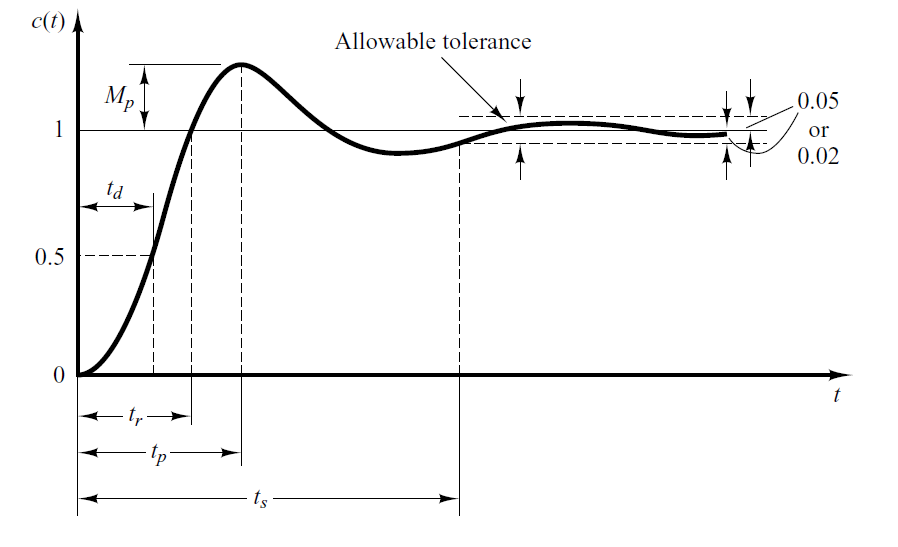
\includegraphics[scale=0.5]{img/transient_ogata_p170}
  \end{center}
  \fonte{Adaptado de \citeonline{Ogata}.} 
  \label{fig:transient_ogata_p170}
\end{figure}

A resposta ao degrau nos diz muito sobre os sistemas de interesse, pois nela podemos ver claramente a atuação dos \textit{polos} e \textit{zeros} dominantes e o ganho de baixa frequência da função de transferência do sistema. Os métodos clássicos para se calcular os parâmetros de controladores são baseados na resposta ao degrau \citeonline{Ogata}. 

%%%%%%%%%%%%%%%%%%%%%%%%%%%%%%%%%%%%%%%%%%%%%%%%%%%%%%%%%%%%%%%%%%%%%%
\section{Controladores}

\begin{figure}[htb]
  \caption{Representação do Modelo de Controlador com distúrbios \textit{l} e \textit{n}.}
  \begin{center}
      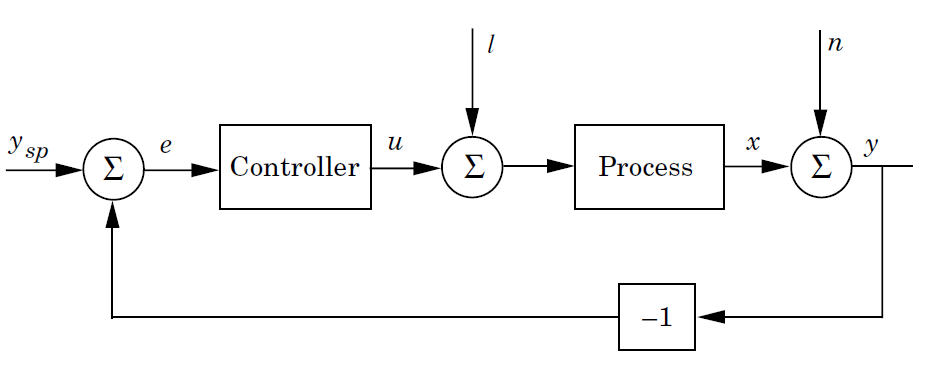
\includegraphics[scale=0.65]{img/feedback_loop_astrom_p65}
  \end{center}
  \fonte{Adaptado de \citeonline{Astrom1995}.} 
  \label{fig:feedback_loop_astrom_p65}
\end{figure}


%%%%%%%%%%%%%%%%%%%%%%%%%%%%%%%%%%%%%%%%%%%%%%%%%%%%%%%%%%%%%%%%%%%%%%
\subsection{Sintonia de Controladores}


%%%%%%%%%%%%%%%%%%%%%%%%%%%%%%%%%%%%%%%%%%%%%%%%%%%%%%%%%%%%%%%%%%%%%%
\subsection{Controladores PID}

\begin{figure}[htb]
  \caption{Representação do Modelo de Controlador PID com distúrbios.}
  \begin{center}
      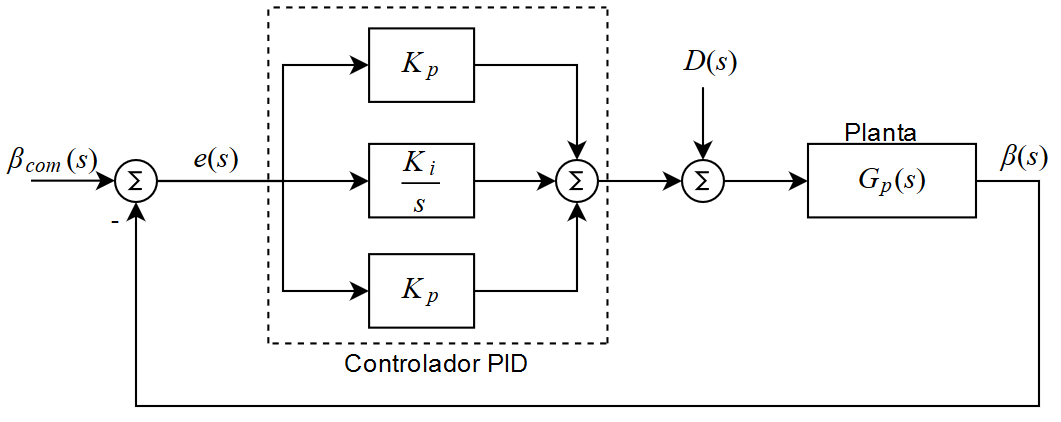
\includegraphics[scale=0.75]{img/pid_controller_Snider_p35}
  \end{center}
  \fonte{\citeonline{Snider}.} 
  \label{fig:pid_controller_Snider_p35}
\end{figure}

\begin{figure}[htb]
  \caption{Modelo de um Controlador com Auto-sintonia.}
  \begin{center}
      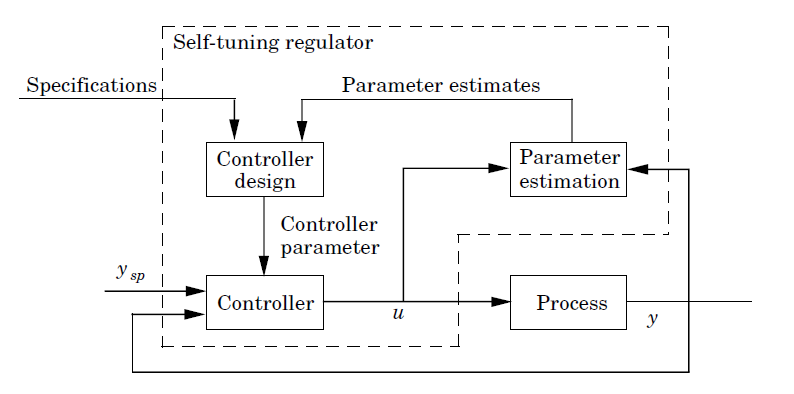
\includegraphics[scale=0.75]{img/pid_adaptative_astrom_p233}
  \end{center}
  \fonte{Adaptado de \citeonline{Astrom1995}.} 
  \label{fig:pid_adaptative_astrom_p233}
\end{figure}

\begin{figure}[htb]
  \caption{Modelo de um Controlador PID com Histerese}
  \begin{center}
      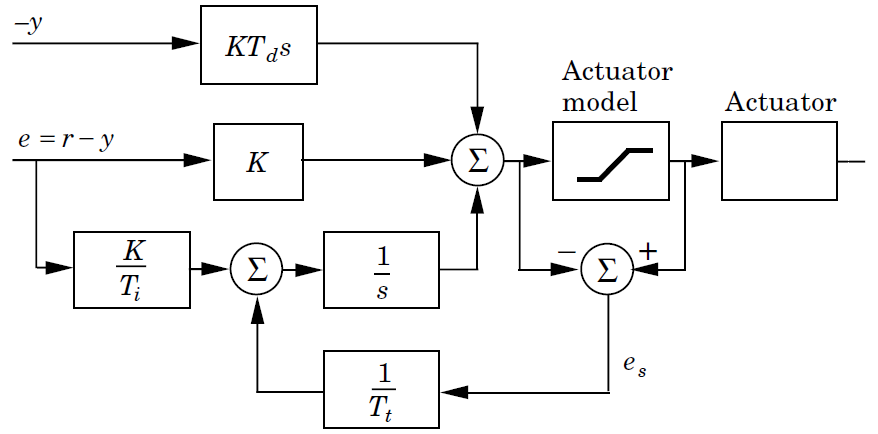
\includegraphics[scale=0.65]{img/pid_antiwindup_astrom_p83}
  \end{center}
  \fonte{Adaptado de \citeonline{Astrom1995}.} 
  \label{fig:pid_antiwindup_astrom_p83}
\end{figure}

\begin{figure}[htb]
  \caption{Modelo do Método de Auto Sintonia via Relé.}
  \begin{center}
      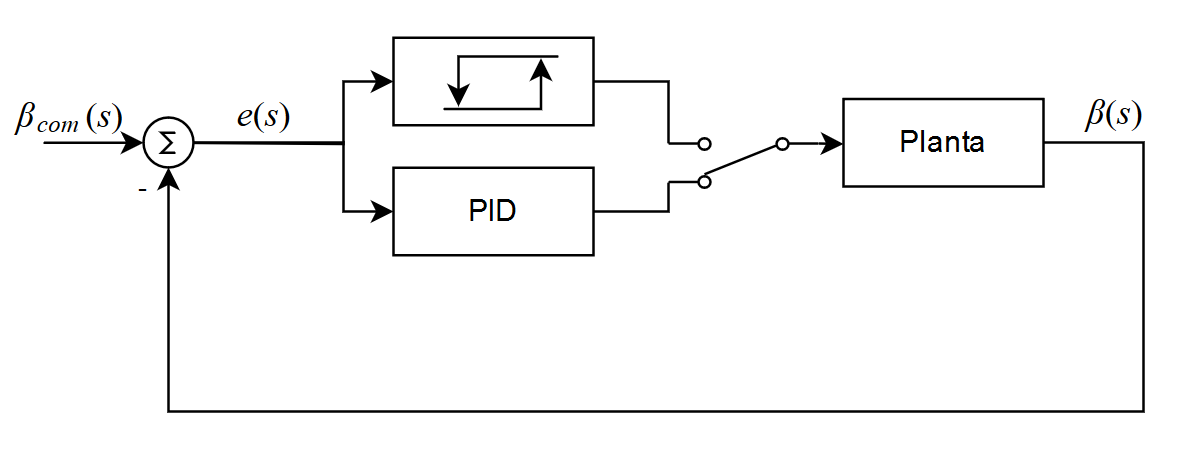
\includegraphics[scale=0.75]{img/pid_autotuning_relay_astrom_p239}
  \end{center}
  \fonte{Adaptado de \citeonline{Astrom1995}.} 
  \label{fig:pid_autotuning_relay_astrom_p239}
\end{figure}

%%%%%%%%%%%%%%%%%%%%%%%%%%%%%%%%%%%
\subsection{Método de sintonia de Ziegler-Nichols}

%%%%%%%%%%%%%%%%%%%%%%%%%%%%%%%%%%%
\subsection{Outras configurações de controladores PID}

%%%%%%%%%%%%%%%%%%%%%%%%%%%%%%%%%%%%%%%%%%%%%%%%%%%%%%%%%%%%%%%%%%%%%%
\section{Controle Inteligente}

%%%%%%%%%%%%%%%%%%%%%%%%%%%%%%%%%%%
\subsection{Lógica Fuzzy}

%%%%%%%%%%%%%%%%%%%%%%%%%%%%%%%%%%%
\subsection{Controle com Redes Neurais}  %control hand p1017

%%%%%%%%%%%%%%%%%%%%%%%%%%%%%%%%%%%%%%%%%%%%%%%%%%%%%%%%%%%%%%%%%%%%%%
\section{Satélites}

\begin{figure}[htb]
  \caption{Representação do Modelo de Controlador PI com dois motores.}
  \begin{center}
      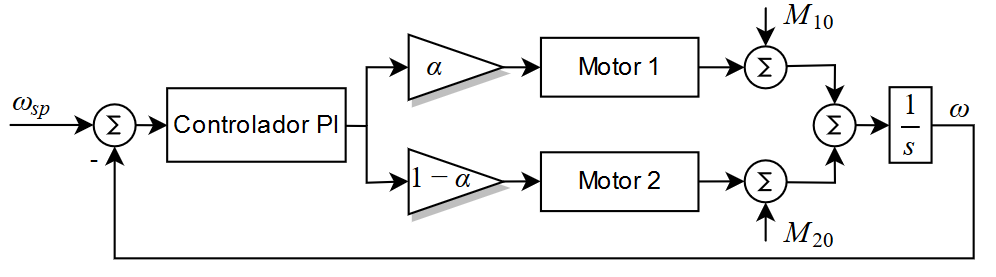
\includegraphics[scale=0.65]{img/pi_twomotors_astrom_p308}
  \end{center}
  \fonte{Adaptado de \citeonline{Astrom1995}.} 
  \label{fig:pi_twomotors_astrom_p308}
\end{figure}

%%%%%%%%%%%%%%%%%%%%%%%%%%%%%%%%%%%
\subsection{Dinâmica rotacional de um Satélite}

\begin{figure}[htb]
  \caption{Representação Mecânica Simplificada de um satélite com rodas de Reação.}
  \begin{center}
      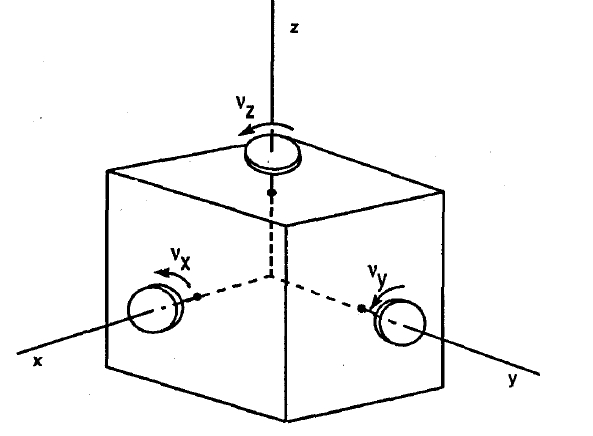
\includegraphics[scale=0.75]{img/satellite_controlhand_p1306}
  \end{center}
  \fonte{Adaptado de \citeonline{Levine1996}.} 
  \label{fig:satellite_controlhand_p1306}
\end{figure}

%%%%%%%%%%%%%%%%%%%%%%%%%%%%%%%%%%%%%%%%%%%%%%%%%%%%%%%%%%%%%%%%%%%%%%
\section{Sistemas Embarcados}

\begin{figure}[htb]
  \caption{Estrutura Básica do Espaço de Usuário e de Kernel.}
  \begin{center}
      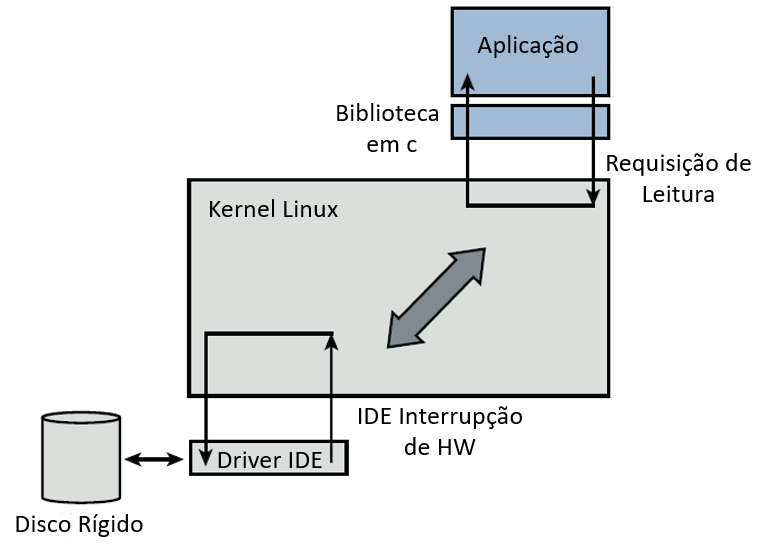
\includegraphics[scale=0.75]{img/kernel_user_space}
  \end{center}
  \fonte{Adaptado de Embarcados....} 
  \label{fig:kernel_user_space}
\end{figure}


\begin{figure}[htb]
  \caption{Representação do Modelo de Controlador PID com distúrbios}
  \begin{center}
      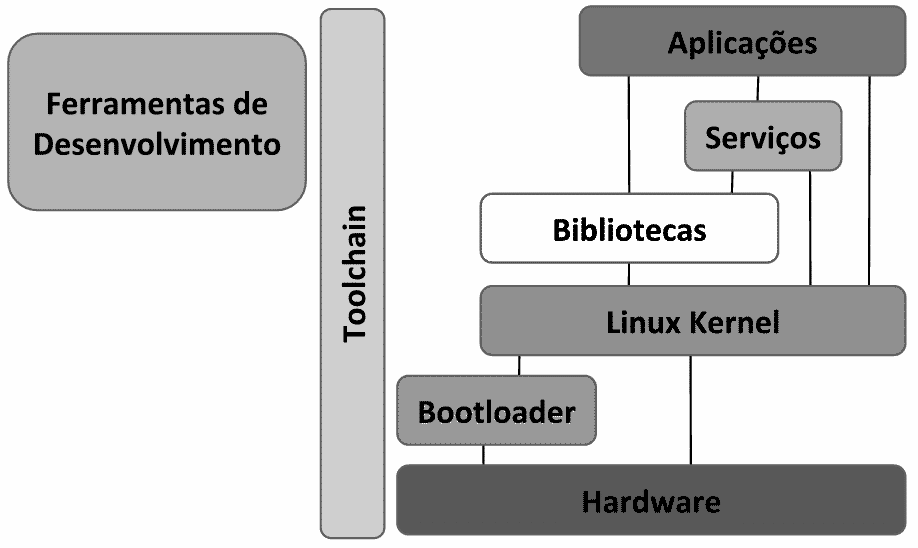
\includegraphics[scale=0.35]{img/sistema-linux-overview_embarcados}
  \end{center}
  \fonte{Adaptado de Embarcados....} 
  \label{fig:sistema-linux-overview_embarcados}
\end{figure}

\begin{figure}[htb]
  \caption{Resposta ao degrau com diferentes períodos de amostragem.}
  \begin{center}
      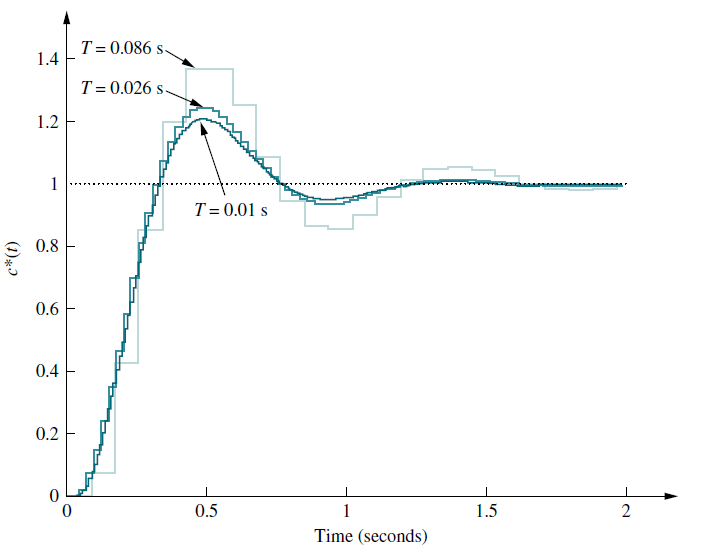
\includegraphics[scale=0.65]{img/nise_digitalinput_p761}
  \end{center}
  \fonte{Adaptado de \citeonline{Nise}.} 
  \label{fig:nise_digitalinput_p761}
\end{figure}

%%%%%%%%%%%%%%%%%%%%%%%%%%%%%%%%%%%
\subsection{Comportamento Assíncrono}

%%%%%%%%%%%%%%%%%%%%%%%%%%%%%%%%%%%
\subsection{Threds}

%%%%%%%%%%%%%%%%%%%%%%%%%%%%%%%%%%%%%%%%%%%%%%%%%%%%%%%%%%%%%%%%%%%%%%
\section{Estado da Arte}

%%%%%%%%%%%%%%%%%%%%%%%%%%%%%%%%%%%
\subsection{Sistemas Inteligentes de Sintonia de Controladores}

\begin{figure}[htb]
  \caption{Modelo de um Simples Neurônio.}
  \begin{center}
      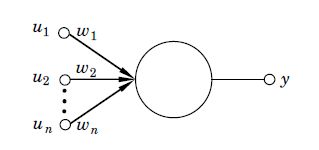
\includegraphics[scale=0.6]{img/neuron_astrom_p295}
  \end{center}
  \fonte{Adaptado de \citeonline{Astrom1995}.} 
  \label{fig:neuron_astrom_p295}
\end{figure}

\begin{figure}[htb]
  \caption{Representação de uma Rede Neural.}
  \begin{center}
      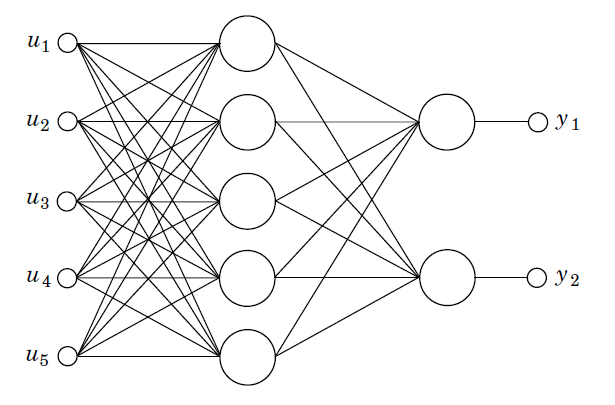
\includegraphics[scale=0.65]{img/feedforward_neural_astrom_p297}
  \end{center}
  \fonte{Adaptado de \citeonline{Astrom1995}.} 
  \label{fig:feedforward_neural_astrom_p297}
\end{figure}

\begin{figure}[htb]
  \caption{Proposta de \citeonline{Chen2004} para um Controlador PID com Redes Neurais}
  \begin{center}
      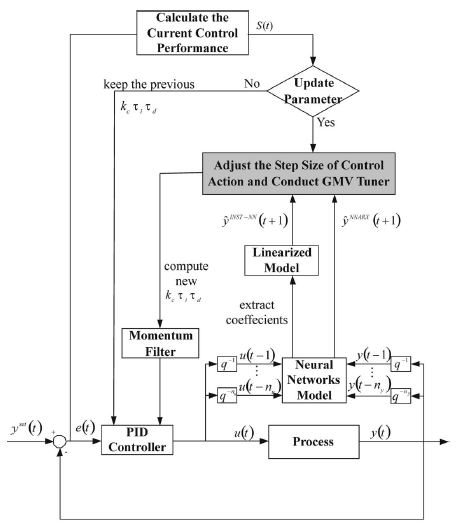
\includegraphics[scale=1]{img/pid_neural_Applying_p18}
  \end{center}
  \fonte{Adaptado de \citeonline{Chen2004}.} 
  \label{fig:pid_neural_Applying_p18}
\end{figure}

%%%%%%%%%%%%%%%%%%%%%%%%%%%%%%%%%%%%%%%%%%%%%%%%%%%%%%%%%%%

\cite{Verma2018}
\cite{Li2010}
\cite{Nise}
\cite{Chen2004}
\cite{Liguo2008}
\cite{Amaral}
\cite{Araari2014}
\cite{Rolle2009}
\cite{Li}
\cite{Ogata}
\cite{Snider}
\cite{Gohiya2012}
\cite{Hu2001}
\cite{Johnson}
\cite{Editor}
\cite{Li2013}
\cite{Das2017}
\cite{Dorf}
\cite{Levine1996}
\cite{Thomas}
\cite{Guo2010}
\cite{Liu2011}
\cite{Astrom1995}
\cite{Behera2017}